\documentclass[10pt,a4paper]{article}
\usepackage[utf8]{inputenc}
\usepackage[english]{babel}
\usepackage{amsmath}
\usepackage{amsfonts}
\usepackage{amssymb}
\usepackage{graphicx}
\usepackage[margin=0.4in]{geometry}
%\usepackage[demo]{graphicx} % "demo" option just for this example
\usepackage{subcaption}
\begin{document}
\section{Parameter Estimation}
\begin{center}
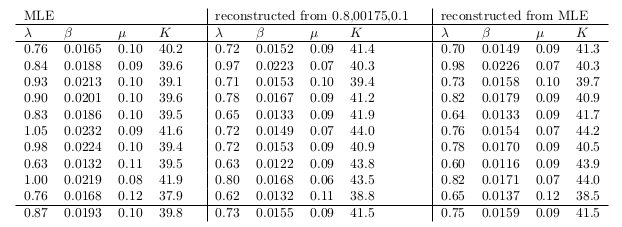
\includegraphics[scale=0.8]{table1.png}
\end{center}
\section{Example (seed 7)}
\begin{figure}[t!] % "[t!]" placement specifier just for this example
\begin{subfigure}{0.48\textwidth}
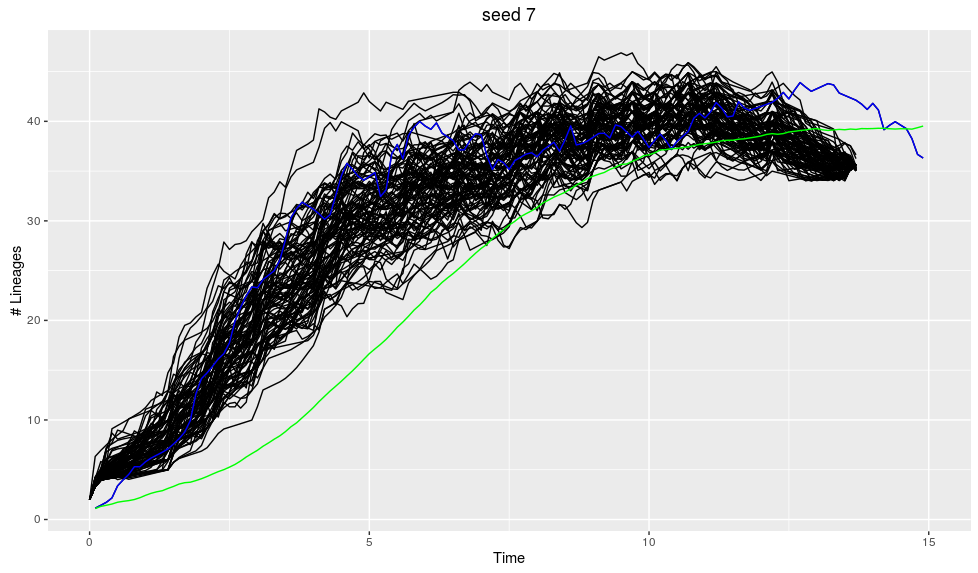
\includegraphics[width=\linewidth]{ph3.png}
\caption{LTT plot. In blue the real tree.} \label{fig:a}
\end{subfigure}\hspace*{\fill}
\begin{subfigure}{0.48\textwidth}
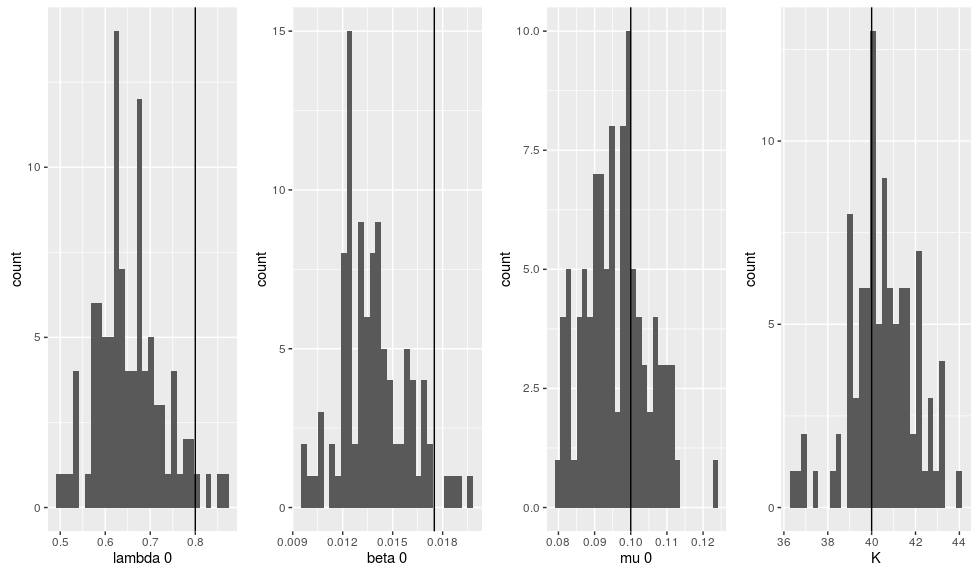
\includegraphics[width=\linewidth]{ph4.png}
\caption{Parameter estimates of reconst trees from real pars} \label{fig:b}
\end{subfigure}

\medskip
\begin{subfigure}{0.48\textwidth}
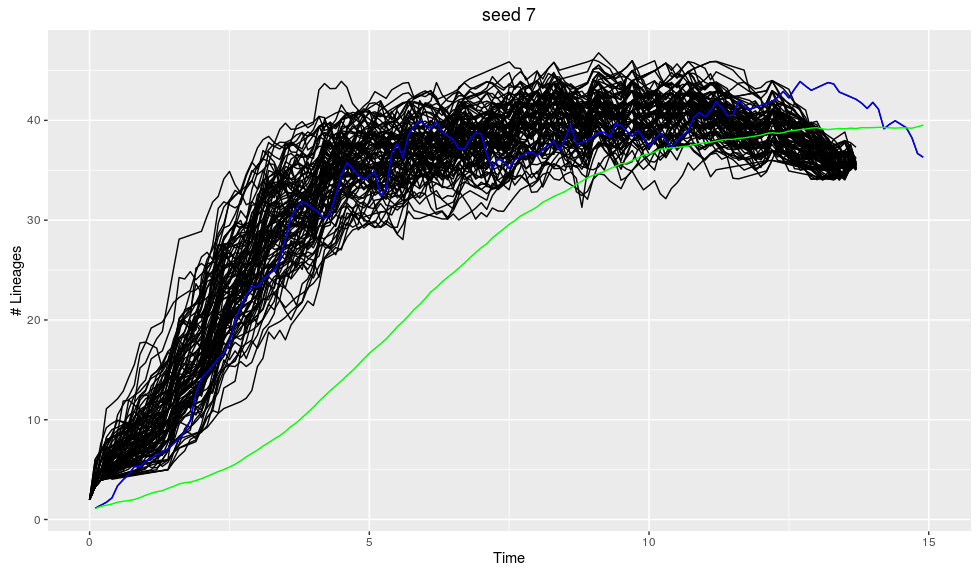
\includegraphics[width=\linewidth]{ph5.png}
\caption{LTT plot.} \label{fig:c}
\end{subfigure}\hspace*{\fill}
\begin{subfigure}{0.48\textwidth}
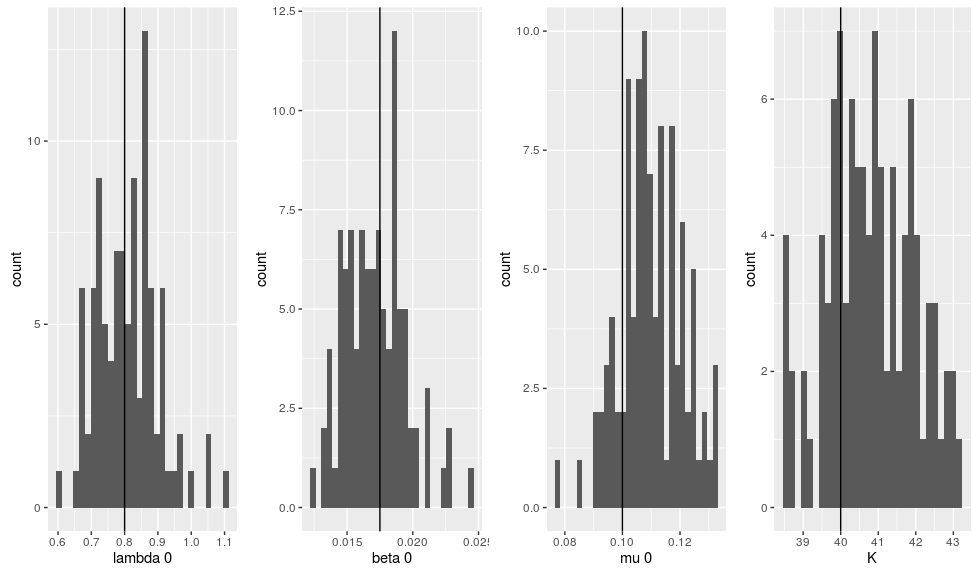
\includegraphics[width=\linewidth]{ph6.png}
\caption{Parameter estimates of reconst trees from real MLE} \label{fig:d}
\end{subfigure}

\medskip
\begin{subfigure}{0.48\textwidth}
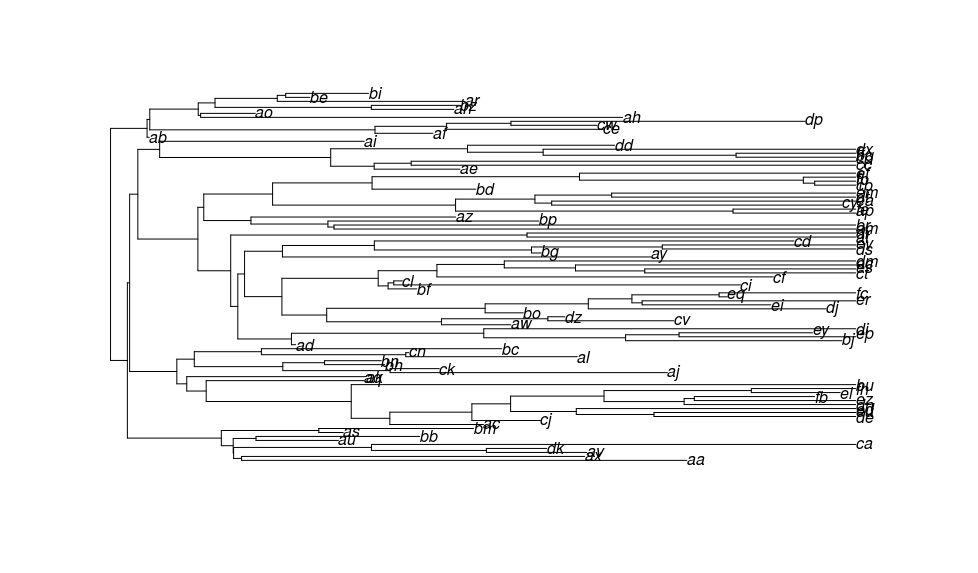
\includegraphics[width=\linewidth]{ph1.png}
\caption{complete phylo tree} \label{fig:e}
\end{subfigure}\hspace*{\fill}
\begin{subfigure}{0.48\textwidth}
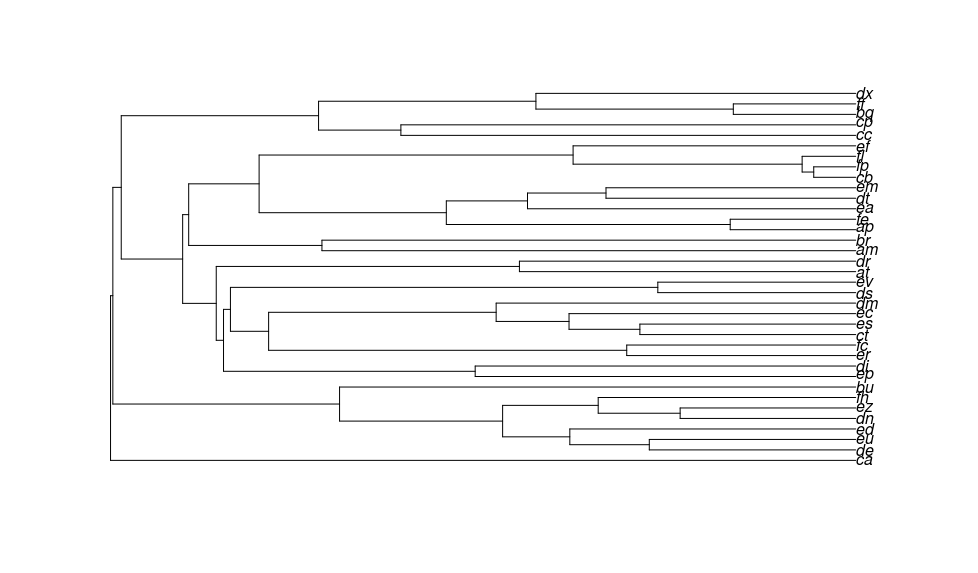
\includegraphics[width=\linewidth]{ph2.png}
\caption{observed phylo tree} \label{fig:f}
\end{subfigure}

%\caption{My complicated figure} \label{fig:1}
\end{figure}
\begin{table}[h!]
\centering
\caption{EM iterations}
\label{my-label}
\begin{tabular}{l|llll}
it & $\lambda$ & $\beta$ & $\mu$ & $K$ \\ \hline
1  & 1.43      & 0.015   & 0.55  & 58  \\
2  & 1.09      & 0.01    & 0.43  & 66  \\
3  & 0.85      & 0.007   & 0.36  & 70  \\
4  & 0.71      & 0.0055  & 0.32  & 71  \\
5  & 0.63      & 0.005   & 0.28  & 69  \\
6  & 0.61      & 0.0055  & 0.25  & 65  \\
7  & 0.59      & 0.006   & 0.23  & 61  \\
8  & 0.57      & 0.0065  & 0.20  & 57  \\
9  & 0.55      & 0.007   & 0.18  & 53  \\
10 & 0.53      & 0.0075  & 0.15  & 50  \\
11 & 0.51      & 0.008   & 0.13  & 47  \\
12 & 0.51      & 0.009   & 0.11  & 44  \\
13 & 0.51      & 0.0095  & 0.10  & 43  \\
14 & 0.49      & 0.0095  & 0.08  & 43  \\
15 & 0.47      & 0.0095  & 0.07  & 42  \\
16 & 0.45      & 0.0095  & 0.06  & 41  \\
17 & 0.43      & 0.0095  & 0.06  & 39  \\
18 & 0.41      & 0.009   & 0.05  & 40  \\
19 & 0.43      & 0.01    & 0.04  & 39  \\
20 & 0.39      & 0.009   & 0.03  & 40  \\
21 & 0.39      & 0.009   & 0.03  & 40  \\
22 & 0.37      & 0.0085  & 0.03  & 40  \\
23 & 0.35      & 0.008   & 0.02  & 41  \\
24 & 0.37      & 0.009   & 0.02  & 39  \\
25 & 0.37      & 0.009   & 0.01  & 39  \\
26 & 0.37      & 0.009   & 0.01  & 40  \\
27 & 0.35      & 0.0085  & 0.01  & 40  \\
28 & 0.35      & 0.0085  & 0.01  & 40  \\
29 & 0.35      & 0.0085  & 0.01  & 40  \\
30 & 0.35      & 0.0085  & 0.01  & 40 
\end{tabular}
\end{table}
\end{document}